\section{Architecture}

ECHOREPO follows a layered architecture in which data acquisition, ingestion, curation, storage and publication are treated as separate concerns. This separation was a deliberate design choice. In the ECHO workflow, citizen observations are collected outside the repository itself, through a mobile application backed by Firebase services and its own authentication model. ECHOREPO therefore does not depend on the internal structure of the collection application. Instead, it acts as an independent research-data infrastructure that receives external data, harmonises them, preserves provenance and produces reusable canonical outputs.

Figure~\ref{fig:echorepo_architecture} summarises the main architectural layers and data flows.

\begin{figure}[htbp]
    \centering
    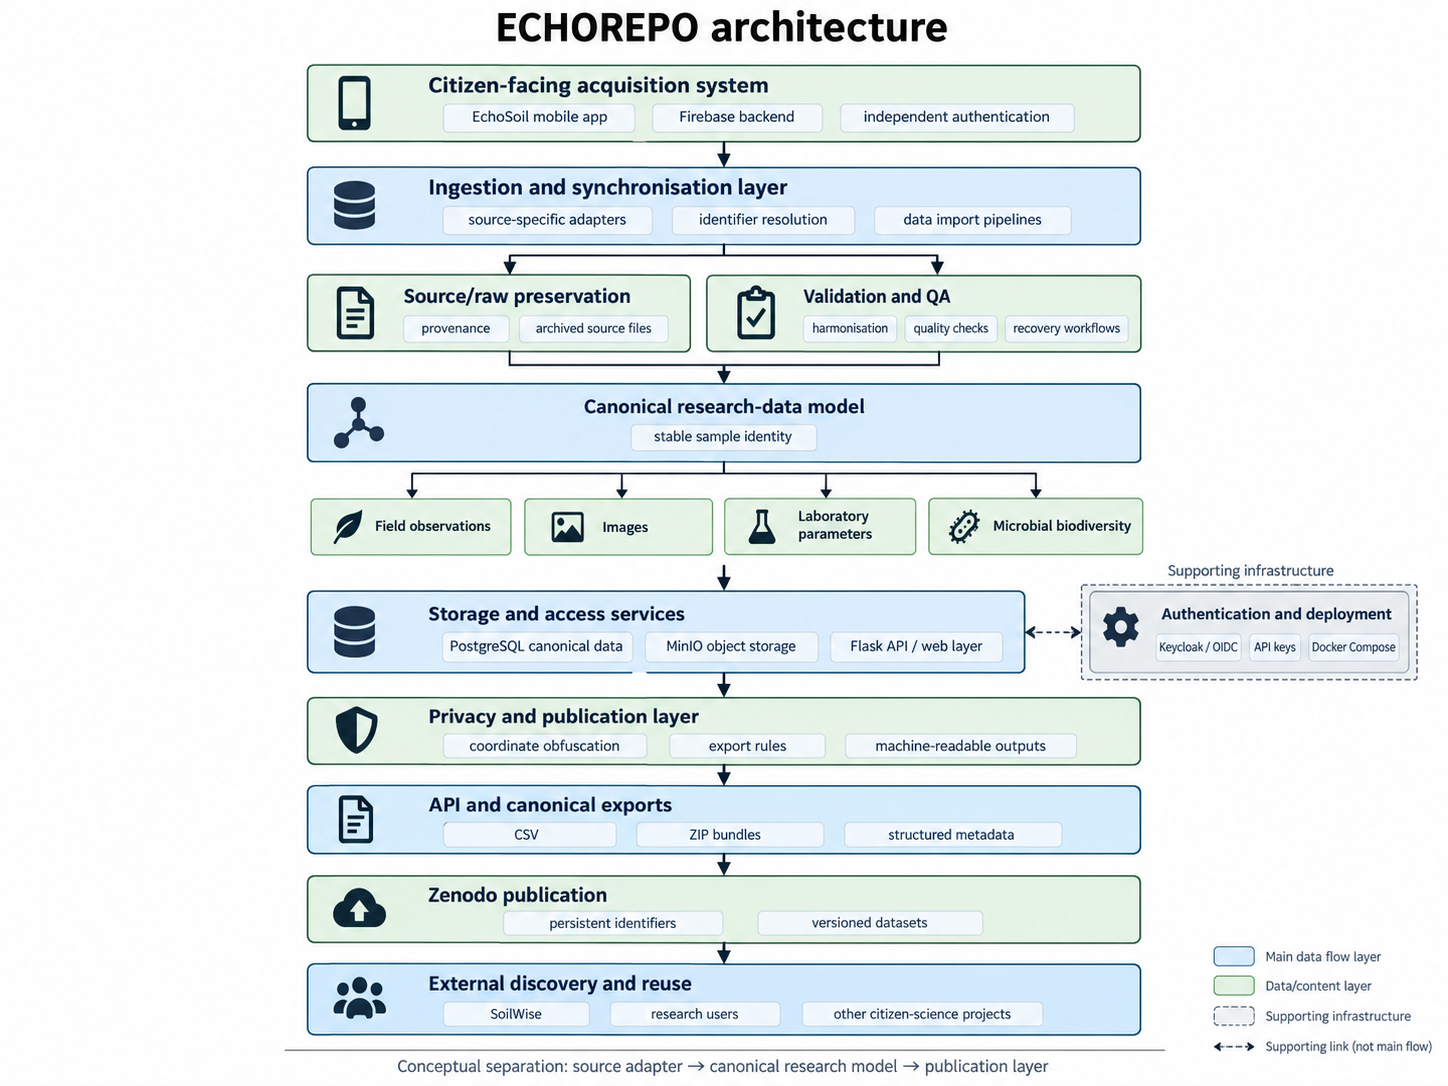
\includegraphics[width=\textwidth]{figures/echorepo_architecture_flowchart.png}
    \caption{Simplified architecture of ECHOREPO. Data are collected in an external citizen-facing system and then pass through ingestion, validation, canonicalisation, enrichment, storage and publication layers before being exposed through APIs and deposited in Zenodo for long-term FAIR dissemination.}
    \label{fig:echorepo_architecture}
\end{figure}

At the upstream end of the workflow, the citizen-facing acquisition system produces field observations, photographs and sample identifiers. These source records are imported into ECHOREPO through ingestion routines that act as adapters between the external application and the repository. A key architectural principle is that these adapters are source-specific,
while the rest of the repository is designed around a source-decoupled
canonical model. This design is intended to allow the acquisition front
end to be replaced or additional collection systems to be connected
without redesigning the downstream repository.

After ingestion, source records are preserved and subjected to validation and quality-assurance procedures. These procedures include identifier reconciliation, coordinate checking, harmonisation of heterogeneous fields, and recovery-oriented treatment of problematic citizen-generated data. Rather than simply discarding inconsistent records, ECHOREPO attempts to retain traceability and recover useful information whenever possible. This is particularly important in citizen-science settings, where data quality problems are common but often partially correctable.

The core of the system is the canonical sample model, which provides a stable representation of each sample and its associated resources. Around this core, ECHOREPO organises several linked data domains: citizen-observation attributes, sample images, laboratory parameters and microbial biodiversity data. The common sample identity maintained across these domains is essential for integrating heterogeneous evidence generated at different stages of the project.

The current implementation uses Flask for the web application and API layer, PostgreSQL for canonical structured data, and MinIO-compatible object storage for large files and immutable resources. Authentication and protected API access are handled through Keycloak/OpenID Connect together with API-key-based access mechanisms. Docker Compose is used to support reproducible deployment and operational portability. These technologies are implementation choices rather than conceptual requirements, but they demonstrate that the architecture can be realised entirely with widely available open-source components.

Before publication, canonical outputs are filtered through privacy and dissemination rules. In particular, geographical information may be obfuscated to reduce re-identification risk while retaining analytical usefulness. The resulting machine-readable resources are then exposed through the ECHOREPO API and export services, and published to Zenodo with persistent identifiers and structured metadata. This publication layer supports downstream discovery through external infrastructures such as SoilWise.

From a reuse perspective, the architecture can be understood as three main layers: a source adapter layer, a canonical research-data layer, and a publication layer. For another citizen-science project, the source adapters and parts of the canonical schema would likely need domain-specific modification, whereas much of the storage, provenance, authentication, API, publication and deployment infrastructure could be reused with comparatively limited change.